%
% The first command in your LaTeX source must be the \documentclass command.
\documentclass[sigconf]{acmart}

%
% defining the \BibTeX command - from Oren Patashnik's original BibTeX documentation.
\def\BibTeX{{\rm B\kern-.05em{\sc i\kern-.025em b}\kern-.08emT\kern-.1667em\lower.7ex\hbox{E}\kern-.125emX}}
    
% Rights management information. 
% This information is sent to you when you complete the rights form.
% These commands have SAMPLE values in them; it is your responsibility as an author to replace
% the commands and values with those provided to you when you complete the rights form.
%
% These commands are for a PROCEEDINGS abstract or paper.
\copyrightyear{2018}
\acmYear{2018}
\setcopyright{acmlicensed}
\acmConference[CU Boulder '19]{CU Boulder '19: CSCI 4502 - Data Mining}{Fall, 2019}{Boulder, CO}
\acmBooktitle{CU Boulder '19: CSCI 4502 - Data Mining, Fall, 2019, Boulder, CO}
\acmPrice{0.00}

%
% These commands are for a JOURNAL article.
%\setcopyright{acmcopyright}
%\acmJournal{TOG}
%\acmYear{2018}\acmVolume{37}\acmNumber{4}\acmArticle{111}\acmMonth{8}
%\acmDOI{10.1145/1122445.1122456}

%
% Submission ID. 
% Use this when submitting an article to a sponsored event. You'll receive a unique submission ID from the organizers
% of the event, and this ID should be used as the parameter to this command.
%\acmSubmissionID{123-A56-BU3}

%
% The majority of ACM publications use numbered citations and references. If you are preparing content for an event
% sponsored by ACM SIGGRAPH, you must use the "author year" style of citations and references. Uncommenting
% the next command will enable that style.
%\citestyle{acmauthoryear}

%
% end of the preamble, start of the body of the document source.
\begin{document}

%
% The "title" command has an optional parameter, allowing the author to define a "short title" to be used in page headers.
\title{World of Warcraft Classic: Auction House Strategy Analysis}

%
% The "author" command and its associated commands are used to define the authors and their affiliations.
% Of note is the shared affiliation of the first two authors, and the "authornote" and "authornotemark" commands
% used to denote shared contribution to the research.
\author{Nikolai Alexander}
\affiliation{%
\department{CSCI 4502}
  \institution{University of Colorado, Boulder}
  \city{Boulder}
  \state{CO}
  \country{USA}}
\email{nial3328@colorado.edu}

%
% By default, the full list of authors will be used in the page headers. Often, this list is too long, and will overlap
% other information printed in the page headers. This command allows the author to define a more concise list
% of authors' names for this purpose.
\renewcommand{\shortauthors}{Alexander}

%
% The abstract is a short summary of the work to be presented in the article.
\begin{abstract}
I am analyzing different characteristics of the World of Warcraft Classic (WoW Classic) economy to determine if there is predictability in the behavior. The in-game auction house is the benchmark for all tradable item prices in the game, do to it overwhelmingly being the most popular form of trading amongst players. I have written a script to periodically scan the auction house, and extract the data to an AWS server. My primary analysis completed so far includes correlations between craftable items and their respective materials and weekly price trends of items classified as trade goods. My future work on this project is going to be a deeper dive into the behavior of consumable trade goods including logistic regression on the direction of the market.
\end{abstract}

%
% The code below is generated by the tool at http://dl.acm.org/ccs.cfm.
% Please copy and paste the code instead of the example below.
%
\begin{CCSXML}
<ccs2012>
<concept>
<concept_id>10002950.10003648.10003704</concept_id>
<concept_desc>Mathematics of computing~Multivariate statistics</concept_desc>
<concept_significance>500</concept_significance>
</concept>
<concept>
<concept_id>10002951.10002952.10002953.10002955</concept_id>
<concept_desc>Information systems~Relational database model</concept_desc>
<concept_significance>300</concept_significance>
</concept>
</ccs2012>
\end{CCSXML}

\ccsdesc[500]{Mathematics of computing~Multivariate statistics}
\ccsdesc[300]{Information systems~Relational database model}

%
% Keywords. The author(s) should pick words that accurately describe the work being
% presented. Separate the keywords with commas.
\keywords{Video Game Economy Analysis, Economic Trend Prediction, World of Warcraft Classic, Auction House}

%
% This command processes the author and affiliation and title information and builds
% the first part of the formatted document.
\maketitle

\section{Introduction}
World of Warcraft Classic (WoW Classic) is a remake of the original Massive Multiplayer Online Role-Playing Game (MMORPG), World of Warcraft, released on November 23, 2004. Within this game, players can complete quests, explore dungeons, and trade with non-player characters (NPCs) and fellow players. One of the major aspects of WoW classic is its complex economy, specifically its auction house. The auction house is a trading hub that allows players to buy and sell items with each other for a price set by the seller. Pricing is competitive and volatile, with players continuously undercutting and buying out each other in an attempt to gain the most profit from their items. Prices can be affected by many factors, such as popularity of the item, relevance to current content, and popular weekly routines of the player-base. Price fluctuations also have an element on randomness to them due to the freedom of the market.
	The premise is my project to find any predictability within the in-game stock market that can be harnessed for both short- and long-term investments in items. All of these supports the goal of a deeper understanding of in-game economies. Like the real-world stock market, economies within MMORPG’s contain abstract behavior stemming from human behavior – Some items have very high volatility related to content within the game, and some items have prices that barely change over time. 

\begin{figure}[h]
  \centering
  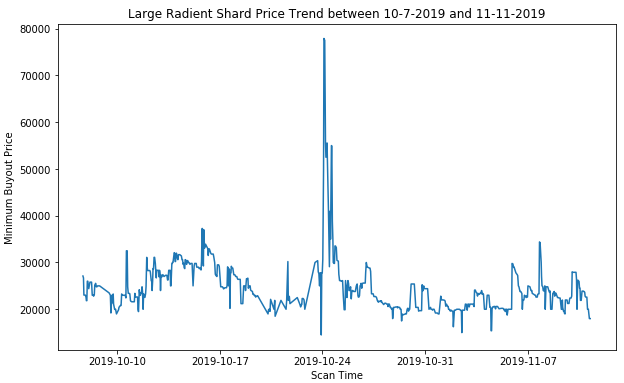
\includegraphics[width=\linewidth]{LRS_Price_Trend}
  \caption{Price trend of Large Radiant Shard between 10/7/2019 and 11/11/2019}
  \Description{Price trend of Large Radiant Shard between 10/7/2019 and 11/11/2019}
\end{figure}

	Because there is no public data on the WoW Classic Auction House, I am required to produce my own data set. I have written a script which I have running on a home-made server that perpetually scans the auction house data and uploads it to an AWS database. This allows for an easy form of passive data collection that I can use for my analysis. The script was deployed on 10/7 at 4 pm MST and as of 11/13 the database consists of 749 scans of 5887 items. The next steps in the project is exploratory analysis on certain aspects of the auction house. Such analysis includes correlations between craftable items and their materials, regression price trends, the behavior of high volatility items, and explanations for outliers. So far correlation analysis had been done between craftable Best-in-Slot (BiS) items and their respective materials, and I am beginning to explore weekly price trends for certain items. Lastly, I plan on doing logistic regression to predict the future direction of the prices on the auction house.

\section{Project Checkpoint}

\subsection{Data Collection}

	I have deployed the script to extract the auction house data from WoW Classic’s game files. The script is running on an old computer perpetually scanning the most recent auction house data and looking for updates (Figure 2). To access the game data, I am using a licensed addon called TradeSkillMaster (TSM) which scans the auction house periodically. Because WoW Classic does not have any publicly accessible API, TSM relies on players in the game to manually scan the auction house using the in-game app. This data is then uploaded to an external program which syncs will all other players using the app. Because many players use this app, it updates rather frequently. The updated data is stored in the game files, in a file called AppData.lua. Every time AppData.lua updates, my script parses and cleans the data and pushes it to an AWS postgres database. 

\begin{figure}[h]
  \centering
  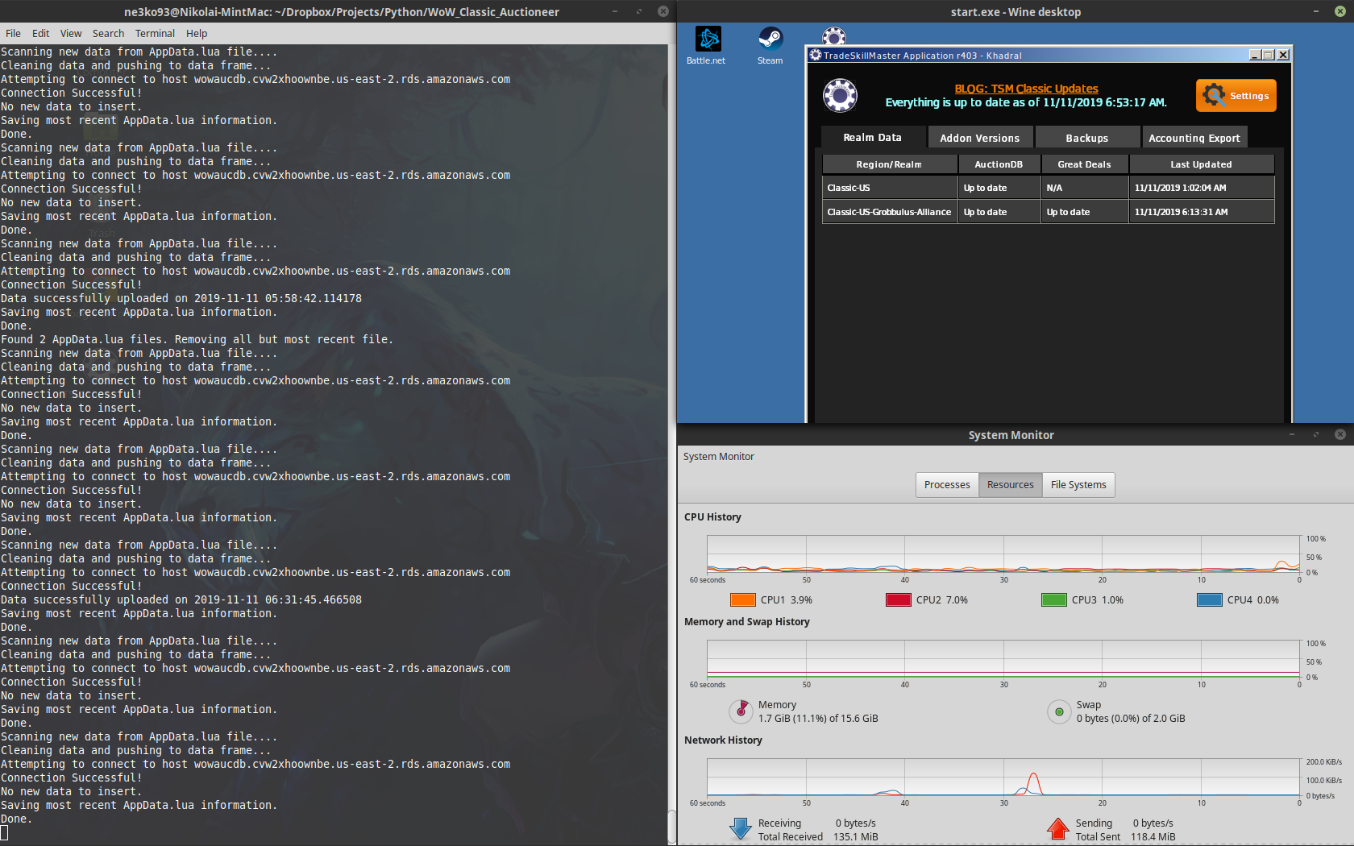
\includegraphics[width=\linewidth]{Server_Screenshot}
  \caption{Screenshot of server running data parsing script.}
  \Description{Screenshot of server running data parsing script.}
\end{figure}

\subsection{Correlation Analysis}

So far I have done correlation analysis on the craftable Best-in-Slot (BiS) gear and their respective materials. I have looked at Green Lens,  Devilsaur Gauntlets, and Devilsaur leggings. Unfortunately, for the most part the materials had little-to-no correlation with the craftable items. My hypothesis on this is that many materials are used to craft many items, leading to quite a bit of disassociation with specific craftables. However, I did find an interesting correlation between Devilsaur Gauntlets and Devilsaur Leggings – They have a strong correlation of 0.52 (Figure 3). I am planning on doing future analysis to see if there are any other factors playing into the correlation of these two items.

\begin{figure}[h]
  \centering
  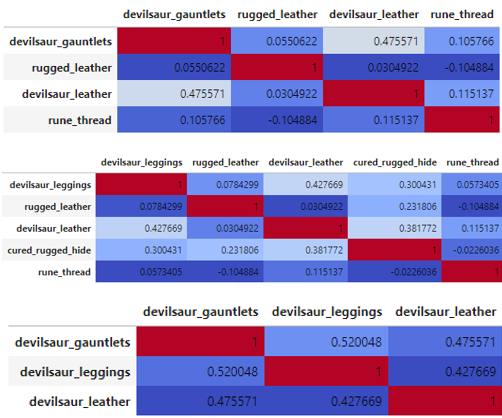
\includegraphics[width=\linewidth]{Devilsaur_Correlations}
  \caption{Correlations between Devilsaur Gauntlets and its crafting materials (top), Devilsaur Leggings and its crafting materials (middle), and between Devilsaur Gauntlets and Devilsaur Leggings (bottom)}
  \Description{Correlations between Devilsaur Gauntlets and its crafting materials (top), Devilsaur Leggings and its crafting materials (middle), and between Devilsaur Gauntlets and Devilsaur Leggings (bottom)}
\end{figure}

\subsection{Weekly Trend – Large Radiant Shard}

The next thing I looked at was weekly trends of the item Large Radiant Shard. The reason I chose this item is because I have been watching quite a bit over the course of a couple weeks and hypothesised that there was in-fact a trend. It also had a random spike in price, where the price increased to almost 4x its value over the course of two days. From a basic five-number-summary, and a scatterplot of the data over the course I have not seen anything that stands out. There looks to be a slight increase price over Wednesday and Thursday and a decrease on Fridays, however not by much.

\begin{figure}[h]
  \centering
  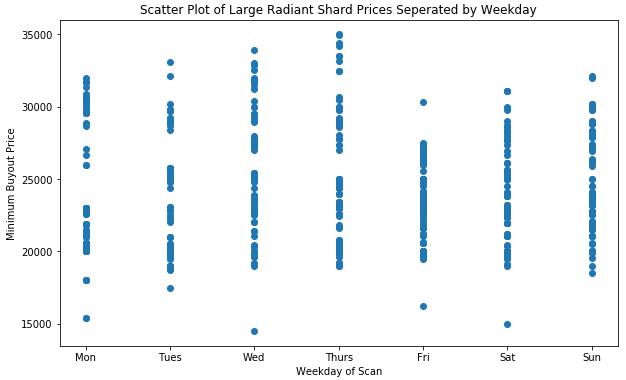
\includegraphics[width=\linewidth]{LRS_Weekly}
  \caption{Scatterplot of Large Radiant Shard Prices spread between the days of the week.}
  \Description{Scatterplot of Large Radiant Shard Prices spread between the days of the week.}
\end{figure}

\section{Further Work}

\subsection{Future Exploratory Analysis}

	Through the analysis I have done so far, I have not found any information that particularly stands out, and have come to the conclusion that I have been looking at the wrong types of items for my goal. Majority of the items I have looked at are one-time buys, such as armor and weapons. This leads to two problems: These items have a very low buy percentage relative to other types of items, and as a result there is very low volatility relative to other items. Enchanting materials perform slightly better. However, enchantments on gear are permanent, so a player generally only gets a particular enchantment once per piece of wearable items.

	My next approach is looking at specific consumable items, or items that a player can use only once. One item in particular is the Greater Fire Protection Potion. One of the major aspects of WoW Classic is the raiding content – A large group of 25 to 40 players get together to infiltrate a massive instance usually resulting in defeating a major antagonist. In the current raiding content, the three major raids are all themed around fire. In order to increase survivability, players need to maximize their fire resistance in every possible way they can. The final boss of The Molten Core, Ragnaros, is virtually impossible to beat without very high fire resistance. As a result, in theory, the rate in which Greater Fire Protection Potion is posted correlates well with the raiding schedule – groups tend to raid more between Tuesday and Thursdays due to the server reset being every Tuesday. Another set of consumables to look at are flasks, such as Flask of the Titans and Flask of Distilled Wisdom. Flasks are extremely powerful potions crafted by players with high Alchemy skills, which are essential in high level content. What makes flasks so important, is their effects last through death. So, if a player consumes Flask of the Titans, their health is guaranteed to increase by 1200 for an hour.

\subsection{Logistic Regression on Price Changes}

Finally, I am planning on using Logistic Regression to predict the direction of the market based on its current values. I am debating between two types of data for this prediction: Daily summaries of the data, or point by point scans of the data. The daily summaries would be structured similarly to a stock market summary. The data set would consist of the opening price (first scan of the day), closing price (last scan of the day), high, low, and volume. The volume is going to be the most difficult of the attributes to figure out, as there is no way of tracking if specific postings are sold. A couple of plans for dealing with this are using the mean number of auctions for the day or the maximum number of auctions for the day. Another shortcoming of this method is that we only have a few instances to work with – So far there is only 39 days’ worth of data. The second method would be taking the raw data and predicting the price change between each scan. The pros of this are that we have much more data to work with (800+ instances rather than 39 instances), and we can more accurately use the number of auctions with each scan. One of the weaknesses to this method is that there is the risk of a much higher level of randomness when predicting price changes on this level, as experienced with predicting the stock market. I am going to experiment with both methods to see which performs better.


\section{Acknowledgments}
I would like to thank Blizzard Entertainment for allowing me to collect data off of World of Warcraft Classic in order to perform this project. I would also like to thank WoWHead for providing me with all of the data and information I need to effectively produce this project.

\section{Honor Code Pledge}
On my honor, as a University of Colorado Boulder student, I have neither given nor received unauthorized assistance. The University of Colorado Honor Code works by receiving the support and participation of all members in the university community. Such an organization is intended to promote a campus culture that consciously upholds the tenets of academic integrity, and moral and ethical conduct.

\section{Citations and Bibliographies}
\begin{enumerate}
	\item Blizzard Entertainment. “Blizzard End User License Agreement.” Blizzard Legal, Blizzard Entertainment, 1 June 2018, www.blizzard.com/en-us/legal/fba4d00f-c7e4-4883-b8b9-1b4500a402ea/blizzard-end-user-license-agreement.
	\item Erorus. “Booty Bay Gazette.” Booty Bay Gazette, The Undermine Journal, 9 Oct. 2019, www.bootybaygazette.com/.
	\item Fanbyte. “World of Warcraft.” Wowhead, 2019, classic.wowhead.com/.
	\item Larrikin, CPP. “Monthly Economic Report - April 2019.” EVE Online, CPP, 13 May 2019, www.eveonline.com/article/prg4uv/monthly-economic-report-april-2019.
	\item “r/Woweconomy.” Reddit, www.reddit.com/r/woweconomy/.
	\item TradeSkillMaster. “Most Advanced Addon for Making Gold in World of Warcraft.” TradeSkillMaster, TradeSkillMaster, 2019, www.tradeskillmaster.com/.
\end{enumerate}

\end{document}
